\subsection{Chi phí giao dịch}

\textit{Gas} là đơn vị thể hiện cho khối lượng tính toán để thực hiện một hành động nào đó trên mạng Ethereum. Do mỗi giao dịch trên mạng Ethereum đều cần tài nguyên tính toán để được thực thi, vì thế mà nó phát sinh ra \textit{chi phí giao dịch}. Khi đó, \textit{gas} thể hiện chi phí để thực hiện giao dịch thành công trên mạng.\\

\begin{figure}[h]
    \centering
    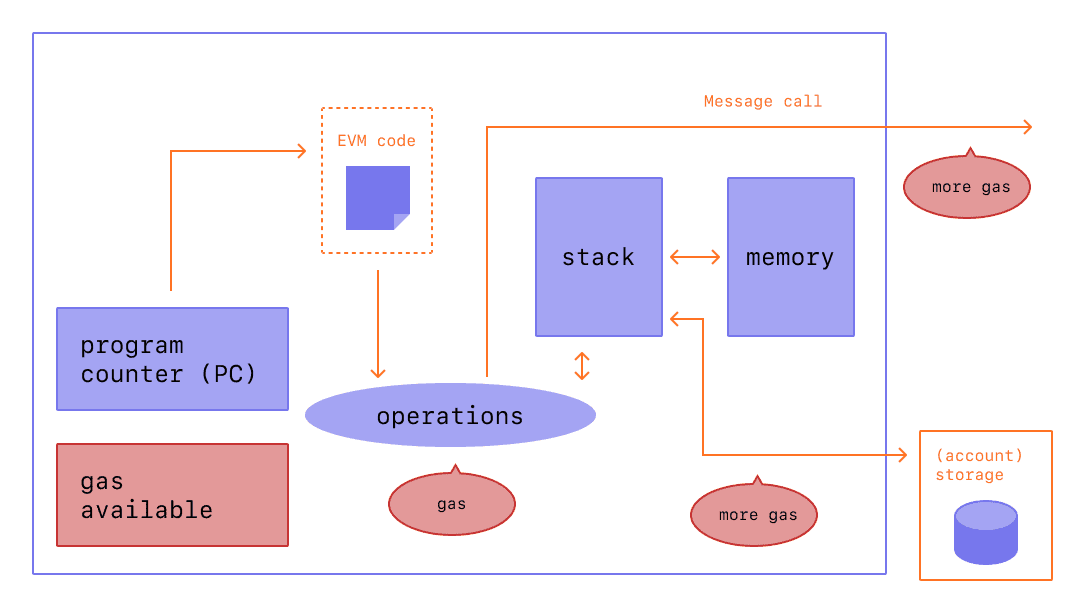
\includegraphics[width=400px]{images/gas.png}
\end{figure}

\textit{Gas} được trả bằng đồng \textit{ether} (ETH). \textit{Giá gas}\footnote{Gas price} có đơn vị là \textit{gwei}, mỗi \textit{gwei} tương ứng với một phần một tỷ của một \textit{ether}: $1$ \textit{gwei} $=10^{-9}$ \textit{ether}. Vì vậy, thay vì nói chi phí giao dịch là $0,000000001$ \textit{ether}, ta có thể nói giao dịch đó tiêu tốn $1$ \textit{gwei}. Ngoài ra, $1$ \textit{gwei} chính là một tỷ \textit{wei}; \textit{wei} (được đặt tên theo \textit{Wei Dai} - nhà khoa học máy tính nổi tiếng đưa ra lý thuyết về thanh toán bằng tiền mã hoá) là đơn vị nhỏ nhất trên Ethereum.\\

